%%mark = star, diamond, square, otimes
%\documentclass{article}
%\usepackage{pgfplots}
%\usepackage[justification=centering]{caption}
%\pgfplotsset{compat=newest}
%\begin{document}
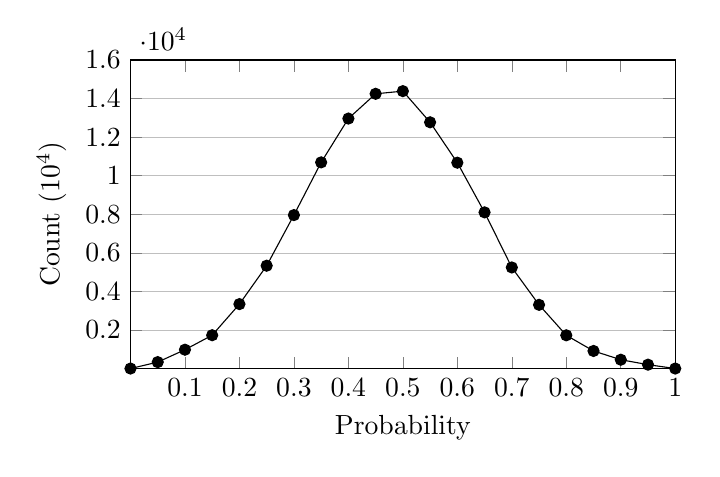
\begin{tikzpicture}
\begin{axis}[
	width=8.5cm,
	height=5.5cm,
    xlabel={Probability },
    ylabel={Count ($10^4$)},
    xmin=0, xmax=1.0,
    ymin=0, ymax=16000,
    xtick={.1,.2,.3,.4,.5,.6,.7,.8,.9,1.0},
    ytick={2000,4000,6000,8000,10000,12000,14000,16000},
    legend pos=north east,
    ymajorgrids=true,
    grid style={line width=.2pt,draw=gray!50},
]
 
\addplot[
    solid, every mark/.append style={solid, fill=black}, mark=*
    ]
    coordinates {
			(0,0)
			(0.05,334)
			(0.1,977)
			(0.15,1729)
			(0.2,3342)
			(0.25,5333)
			(0.3,7958)
			(0.35,10692)
			(0.4,12964)
			(0.45,14247)
			(0.5,14386)
			(0.55,12770)
			(0.6,10675)
			(0.65,8099)
			(0.7,5242)
			(0.75,3304)
			(0.8,1724)
			(0.85,912)
			(0.9,458)
			(0.95,201)
			(1,0)

};
 
\end{axis}
\end{tikzpicture}
%\end{document}